\documentclass[12pt,a4paper]{article}
\usepackage[utf8]{inputenc}
\usepackage[english]{babel}
\usepackage{geometry}
\usepackage{fancyhdr}
\usepackage{graphicx}
\usepackage{longtable}
\usepackage{array}
\usepackage{booktabs}
\usepackage{xcolor}
\usepackage{hyperref}
\usepackage{listings}
\usepackage{enumitem}
\usepackage{caption}
\usepackage{float} % for [H] placement
\geometry{margin=1in}
\pagestyle{fancy}
\fancyhf{}
\rhead{\thepage}
\lhead{HIV Clinic RDS}

\title{\textbf{Requirement \& Design Specification\\HIV Clinic Appointment Booking System}}
\author{Version: 1.0}
\date{January 2025}

\begin{document}

\maketitle
\thispagestyle{empty}

\newpage

\section*{Record of Changes}

\begin{table}[h!]
\centering
\renewcommand{\arraystretch}{1.5}
\begin{tabular}{|c|c|c|c|p{7.5cm}|}
\hline
\textbf{Version} & \textbf{Date} & \textbf{A* M, D} & \textbf{In charge} & \textbf{Change Description} \\
\hline
V1.0 & 28/6 & A & KhoaDDSE196260 & 
Create document \newline
Add requirements, Add actors (1.1) \newline
Design Specification\\
\hline
V1.0 & 28/6 & A & TuanTMSE192397 & 
Add descriptions for guest and admin (1.2.b) \newline
Authentication \& User Management (2.1) \\
\hline
V1.0 & 28/6 & A & DatNTSE194083 & 
Add Use Case Diagram (1.2.a)\newline 
Add Requirement Speciality
\\
\hline
V1.0 & 28/6 & A & AnPPSE196260 & 
Add Use case Table(1.2.1)
Add ScreenFlow Diagram (2.1) \newline
(2.2) Screen Descriptions, Appendix\newline 
Add Requirement Speciality\\
\hline
\end{tabular}
\caption{Version Change Log}
\label{tab:version-log}
\end{table}



\textit{*A - Added M - Modified D - Deleted}

\newpage

\tableofcontents

\newpage

\section{Overview}

\subsection{User Requirements}

\subsubsection{Actors}

The HIV Clinic Appointment Booking System involves four main actors who interact with the system to perform various healthcare-related tasks:

\subsection{Actor Description}

\begin{longtable}{|c||c|p{9cm}|}
\hline
\textbf{No} & \textbf{Actor} & \textbf{Description} \\
\hline
01 & Guest & An unauthenticated individual. Allowed to access public website features such as browsing content, registering for an account, or initiating the login process. \\
\hline
02 & Patient & A registered and authenticated user. Can book appointments (public or private), view their medical history, receive notifications, and access personalized treatment plans. \\
\hline
03 & Doctor & A registered and authenticated medical professional. Can manage their availability, handle appointments and consultations, prescribe ARV or other treatments, and manage related patient notifications. \\
\hline
04 & Admin & A privileged user responsible for system administration. Manages user accounts (Patients and Doctors), handles booking rules and exceptions, and monitors overall system integrity. \\
\hline
05 & Manager & An authenticated user with oversight capabilities. Views system-wide analytics, monitors KPIs related to appointments and treatments, and supports data-driven strategic decisions. \\
\hline
\end{longtable}


\subsubsection{Use Cases}

\paragraph{a. Diagram(s)}

\begin{figure}[H]
\centering
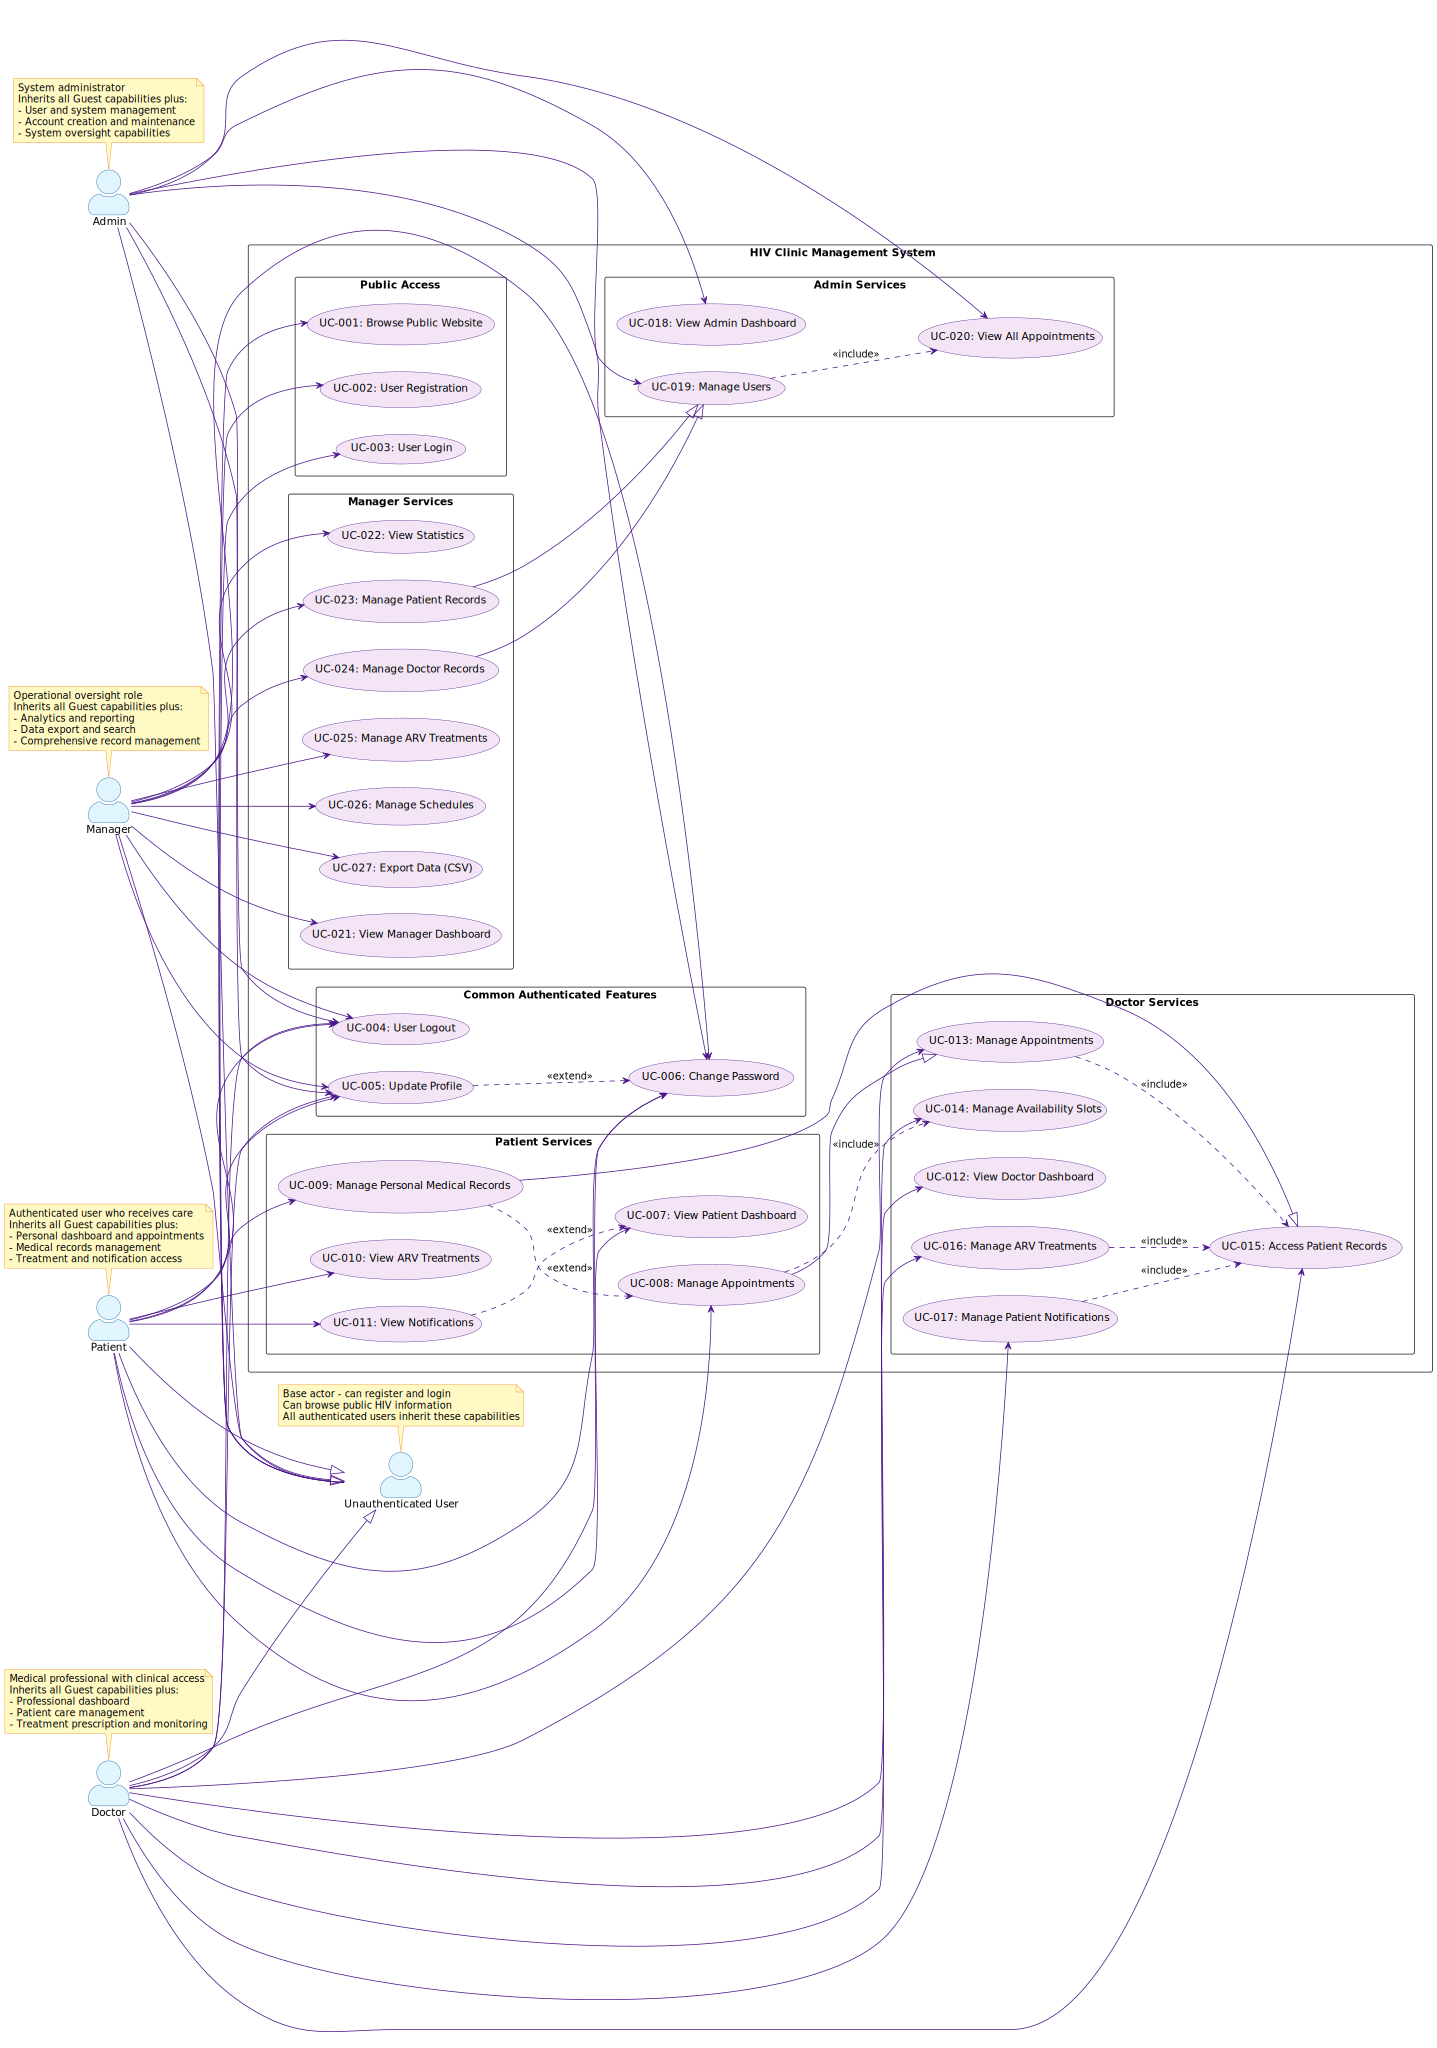
\includegraphics[width=0.9\textwidth]{diagrams/use_case_diagram.png}
\caption{HIV Clinic Management System Use Case Diagram}
\label{fig:use-case-diagram}
\end{figure}

The system provides comprehensive use cases covering patient care, appointment management, and administrative functions for an HIV clinic environment.


% --- Use Case 1 ---
\begin{figure}[H]
    \centering
    \includegraphics[width=0.85\textwidth]{diagrams/Picture/Usecase1.png}
    \caption*{\textbf{Table 1.} Guess Use Case}
\end{figure}

% --- Use Case 2 ---
\begin{figure}[H]
    \centering
    \includegraphics[width=0.85\textwidth]{diagrams/Picture/Usecase2.png}
    \caption*{\textbf{Table 2.} Patient Use Case}
\end{figure}

% --- Use Case 3 ---
\begin{figure}[H]
    \centering
    \includegraphics[width=0.85\textwidth]{diagrams/Picture/Usecase3.png}
    \caption*{\textbf{Table 3.} Doctor Use Case}
\end{figure}

% --- Use Case 4 ---
\begin{figure}[H]
    \centering
    \includegraphics[width=0.85\textwidth]{diagrams/Picture/Usecase4.png}
    \caption*{\textbf{Table 4.} Admin Use Case}
\end{figure}

% --- Use Case 5 ---
\begin{figure}[H]
    \centering
    \includegraphics[width=0.85\textwidth]{diagrams/Picture/Usecase5.png}
    \caption*{\textbf{Table 5.} Manager Use Case}
\end{figure}


\paragraph{b. Descriptions}

\begin{longtable}{|p{1cm}|p{3cm}|p{3cm}|p{7cm}|}
\hline
\textbf{ID} & \textbf{Feature} & \textbf{Use Case} & \textbf{Use Case Description} \\
\hline
\multicolumn{4}{|c|}{\textbf{Authentication \& Profile Management}} \\
\hline
UC-001 & User Management & User Registration & New users (patients/doctors) create accounts with role-based access to the HIV clinic system \\
\hline
UC-002 & Authentication & User Login & Existing users authenticate using username/password with JWT token-based security \\
\hline
UC-003 & Profile Management & Update Profile & Users update personal information, contact details, and profile images \\
\hline
UC-004 & Authentication & Change Password & Users change their account passwords with validation and security checks \\
\hline
UC-005 & Authentication & Logout & Users securely logout from the system and invalidate their session \\
\hline
\multicolumn{4}{|c|}{\textbf{Patient Services}} \\
\hline
UC-006 & Patient Dashboard & View Dashboard & Patients access their personal dashboard with overview of appointments and treatments \\
\hline
UC-007 & Appointment Management & Book Appointment & Patients schedule appointments with available doctors based on doctor availability slots \\
\hline
UC-008 & Appointment Management & View Appointments & Patients view their scheduled, completed, and cancelled appointments with details \\
\hline
UC-009 & Appointment Management & Cancel Appointment & Patients cancel scheduled appointments with cancellation reasons \\
\hline
UC-010 & Patient Care & View Patient Records & Patients access their own medical records, treatment history, and current medications \\
\hline
UC-011 & Patient Care & Update Patient Records & Patients update their personal medical information and emergency contacts \\
\hline
UC-012 & HIV Treatment & View ARV Treatments & Patients view their HIV antiretroviral treatment regimens and adherence status \\
\hline
\multicolumn{4}{|c|}{\textbf{Doctor Services}} \\
\hline
UC-013 & Doctor Dashboard & View Doctor Dashboard & Doctors access their professional dashboard with patient appointments and notifications \\
\hline
UC-014 & Appointment Management & Manage Appointments & Doctors view and manage their scheduled appointments with patients \\
\hline
UC-015 & Appointment Management & Update Appointment Status & Doctors update appointment status (completed, cancelled, rescheduled) \\
\hline
UC-016 & Doctor Operations & Manage Availability Slots & Doctors create, update, and manage their availability time slots for patient appointments \\
\hline
UC-017 & Patient Care & Access Patient Records & Doctors access comprehensive patient medical records during consultations \\
\hline
UC-018 & HIV Treatment & Manage ARV Treatments & Doctors manage HIV antiretroviral treatment regimens, monitor adherence, and track side effects \\
\hline
UC-019 & Notification System & Send Notifications & Doctors send custom notifications to patients regarding appointments and treatments \\
\hline
UC-020 & Notification System & View Notification History & Doctors review history of notifications sent to patients \\
\hline
UC-021 & Notification System & Manage Notification Templates & Doctors create and manage templates for common notifications \\
\hline
\multicolumn{4}{|c|}{\textbf{Admin Services}} \\
\hline
UC-022 & Admin Dashboard & View Admin Dashboard & Administrators access system-wide dashboard with user and system management \\
\hline
UC-023 & User Management & Manage Users & Administrators manage all user accounts across the system \\
\hline
UC-024 & User Management & Manage Patients & Administrators specifically manage patient accounts and information \\
\hline
UC-025 & User Management & Manage Doctors & Administrators manage doctor accounts and professional information \\
\hline
UC-026 & User Management & Create Doctor Accounts & Administrators create new doctor accounts with specialized permissions \\
\hline
UC-027 & User Management & Toggle User Status & Administrators activate or deactivate user accounts across the system \\
\hline
UC-028 & User Management & Reset User Passwords & Administrators reset passwords for users who cannot access their accounts \\
\hline
UC-029 & System Management & Manage Specialties & Administrators manage medical specialties for doctor categorization \\
\hline
UC-030 & System Management & View All Appointments & Administrators view all appointments across the system for oversight \\
\hline
\multicolumn{4}{|c|}{\textbf{Manager Services}} \\
\hline
UC-031 & Manager Dashboard & View Manager Dashboard & Managers access operational dashboard with clinic statistics and analytics \\
\hline
UC-032 & Analytics & View Statistics & Managers view comprehensive clinic statistics and performance metrics \\
\hline
UC-033 & Operations & Manage Patient Records & Managers oversee patient records management and data integrity \\
\hline
UC-034 & Operations & Manage Doctor Records & Managers oversee doctor records and professional information \\
\hline
UC-035 & Operations & Manage ARV Treatments & Managers monitor and oversee ARV treatment programs across the clinic \\
\hline
UC-036 & Operations & Manage Schedules & Managers oversee clinic scheduling and appointment distribution \\
\hline
UC-037 & Search & Search Patients & Managers search for specific patients across the clinic database \\
\hline
UC-038 & Search & Search Doctors & Managers search for specific doctors in the clinic system \\
\hline
UC-039 & Data Export & Export Data (CSV) & Managers export various clinic data in CSV format for reporting and analysis \\
\hline
UC-040 & Detail Views & View Patient Details & Managers access detailed patient information for operational oversight \\
\hline
UC-041 & Detail Views & View Doctor Details & Managers access detailed doctor information for operational oversight \\
\hline
\multicolumn{4}{|c|}{\textbf{Guest Services}} \\
\hline
UC-042 & Public Access & View Home Page & Guests access the public home page with general information about the HIV clinic \\
\hline
UC-043 & Public Access & View Hospital Information & Guests view detailed information about the hospital services and facilities \\
\hline
UC-044 & Public Access & Read Health Blogs & Guests access educational health blogs and articles about HIV/AIDS prevention and care \\
\hline
UC-045 & Public Access & View Contact Information & Guests access contact details and location information for the clinic \\
\hline
UC-046 & Public Access & Access Registration & Guests initiate the account registration process for patients or doctors \\
\hline
\multicolumn{4}{|c|}{\textbf{Advanced Notification Features}} \\
\hline
UC-047 & Notification System & Schedule Automated Notifications & System schedules automated notifications based on appointment and treatment schedules \\
\hline
UC-048 & Notification System & Manage Notification Preferences & Users configure their notification preferences and delivery methods \\
\hline
UC-049 & Notification System & View Notification Analytics & Doctors and managers view analytics on notification delivery and engagement rates \\
\hline
UC-050 & Notification System & Emergency Notifications & System sends emergency notifications to patients and staff during critical situations \\
\hline
UC-051 & Notification System & Bulk Notifications & Administrators send bulk notifications to multiple users simultaneously \\
\hline
\multicolumn{4}{|c|}{\textbf{ARV Treatment Monitoring}} \\
\hline
UC-052 & HIV Treatment & Monitor ARV Adherence & System tracks patient adherence to ARV medication schedules and generates reports \\
\hline
UC-053 & HIV Treatment & Track Side Effects & Doctors and patients record and monitor ARV medication side effects \\
\hline
UC-054 & HIV Treatment & Generate Treatment Reports & System generates comprehensive reports on patient treatment progress and outcomes \\
\hline
UC-055 & HIV Treatment & Manage Drug Interactions & System checks for potential drug interactions with ARV medications \\
\hline
UC-056 & HIV Treatment & Schedule Lab Tests & Doctors schedule regular lab tests for ARV treatment monitoring \\
\hline
\multicolumn{4}{|c|}{\textbf{Session and Security Management}} \\
\hline
UC-057 & Security & Manage User Sessions & System manages user session timeouts and security validations \\
\hline
UC-058 & Security & Two-Factor Authentication & Users enable and use two-factor authentication for enhanced security \\
\hline
UC-059 & Security & Audit Trail & System maintains audit logs of all user activities and data modifications \\
\hline
UC-060 & Security & Data Encryption & System encrypts sensitive patient data and medical records \\
\hline
UC-061 & Security & Access Control & System enforces role-based access control for different user types \\
\hline
\multicolumn{4}{|c|}{\textbf{Advanced Analytics and Reporting}} \\
\hline
UC-062 & Analytics & Generate Clinic Statistics & System generates comprehensive statistics on clinic operations and performance \\
\hline
UC-063 & Analytics & Patient Flow Analysis & Managers analyze patient flow patterns and appointment trends \\
\hline
UC-064 & Analytics & Treatment Outcome Reports & System generates reports on treatment outcomes and success rates \\
\hline
UC-065 & Analytics & Resource Utilization Reports & Managers view reports on doctor availability and resource utilization \\
\hline
UC-066 & Analytics & Financial Reports & System generates financial reports related to appointments and treatments \\
\hline
\multicolumn{4}{|c|}{\textbf{System Administration}} \\
\hline
UC-067 & System Admin & Backup and Recovery & Administrators manage system backups and data recovery procedures \\
\hline
UC-068 & System Admin & System Configuration & Administrators configure system settings and parameters \\
\hline
UC-069 & System Admin & Database Management & Administrators manage database maintenance and optimization \\
\hline
UC-070 & System Admin & System Monitoring & Administrators monitor system performance and health metrics \\
\hline
UC-071 & System Admin & Software Updates & Administrators manage system updates and version control \\
\hline
\multicolumn{4}{|c|}{\textbf{Privacy and Compliance}} \\
\hline
UC-072 & Privacy & Manage Data Consent & Patients manage their data consent preferences and privacy settings \\
\hline
UC-073 & Privacy & Data Anonymization & System anonymizes patient data for research and statistical purposes \\
\hline
UC-074 & Compliance & HIPAA Compliance & System ensures compliance with HIPAA regulations for patient data protection \\
\hline
UC-075 & Compliance & Generate Compliance Reports & System generates reports for regulatory compliance audits \\
\hline
UC-076 & Privacy & Data Retention Management & System manages data retention policies and automatic data purging \\
\hline
\multicolumn{4}{|c|}{\textbf{Integration and External Services}} \\
\hline
UC-077 & Integration & Laboratory Integration & System integrates with external laboratory systems for test results \\
\hline
UC-078 & Integration & Pharmacy Integration & System integrates with pharmacy systems for medication management \\
\hline
UC-079 & Integration & Insurance Integration & System integrates with insurance systems for claim processing \\
\hline
UC-080 & Integration & Telemedicine Integration & System supports telemedicine consultations and virtual appointments \\
\hline
UC-081 & Integration & Electronic Health Records & System integrates with external EHR systems for comprehensive patient records \\
\hline
\end{longtable}
\begin{figure}[H]
    \centering
    
    \caption*{\textbf{Chart 7.} Guest Use Case Diagram}
\end{figure}

\begin{table}[H]
\centering
\renewcommand{\arraystretch}{1.5}
\begin{tabular}{|c|c|c|p{7.5cm}|}
\hline
\textbf{ID} & \textbf{Feature} & \textbf{Use Case} & \textbf{Use Case Description} \\
\hline
01 & Public Access & View Home Page & Guests access the public home page with general information about the HIV clinic. \\
\hline
02 & Public Access & View Hospital Information & Guests view detailed information about the hospital services and facilities. \\
\hline
03 & Public Access & Read Health Blogs & Guests access educational health blogs and articles about HIV/AIDS prevention and care. \\
\hline
04 & Public Access & View Contact Information & Guests access contact details and location information for the clinic. \\
\hline
05 & Public Access & Access Registration & Guests initiate the account registration process for patients or doctors. \\
\hline
06 & Public Access & Access Login & Guests access the login page to authenticate as registered users. \\
\hline
07 & Information & Browse Services & Guests browse available medical services and specialties offered by the clinic. \\
\hline
08 & Information & View Operating Hours & Guests view clinic operating hours and availability information. \\
\hline
09 & Information & Access Emergency Information & Guests access emergency contact information and procedures. \\
\hline
10 & Information & View Privacy Policy & Guests read the clinic's privacy policy and data handling practices. \\
\hline
\end{tabular}
\caption*{\textbf{Table 7.} Guest Use Case Description}
\label{tab:guest-usecases}
\end{table}

\begin{table}[H]
\centering
\renewcommand{\arraystretch}{1.5}
\begin{tabular}{|c|c|c|p{7.5cm}|}
\hline
\textbf{ID} & \textbf{Feature} & \textbf{Use Case} & \textbf{Use Case Description} \\
\hline
01 & Appointment Booking & Manage Appointment & Patient can create appointment and have option to receive notification. \\
\hline
02 & Online Consultation & Online Consultation & Patient books online consultation (can be anonymous) and has online conversation with doctors. \\
\hline
03 & Medical Records & View Patient Record & Patients can view treatment and process. \\
\hline
04 & Personal Information & View Profile & Patients view their personal information (address, phone number, …). \\
\hline
05 & Appointment Booking & Book Appointment & Patient can book an appointment (extends from View Doctors). \\
\hline
06 & Appointments & View Appointments & Patient can view their scheduled appointments. \\
\hline
07 & Appointment Metrics & View Number of Appointments & Patient can see the total number of their appointments. \\
\hline
08 & Notifications & View Notifications & Patient can view notifications sent by the system. \\
\hline
09 & Dashboard Overview & View Dashboard & Patient can access their dashboard to monitor key statistics. \\
\hline
10 & ARV Statistics & View Number of ARV Treatment & Included in Dashboard – shows number of ARV regimens. \\
\hline
11 & Appointment Forecast & View Number of Upcoming Appointments & Included in Dashboard – shows count of upcoming appointments. \\
\hline
12 & Doctor Availability Stats & View Number of Available Doctors & Included in Dashboard – shows available doctors count. \\
\hline
13 & Anonymous Mode & Switch to Anonymous Mode & Patient can switch to anonymous browsing mode. \\
\hline
14 & Profile Viewing & View Personal Profile & Patient can view their personal information. \\
\hline
15 & Profile Updating & Update Personal Profile & Patient can update their personal profile (extends from View Personal Profile). \\
\hline
\end{tabular}
\caption*{\textbf{Table 8.} Patient Use Case Description}
\label{tab:patient-usecases}
\end{table}

\renewcommand{\arraystretch}{1.5}
\begin{longtable}{|c|c|c|p{7.5cm}|}
\hline
\textbf{ID} & \textbf{Feature} & \textbf{Use Case} & \textbf{Use Case Description} \\
\hline
\endfirsthead

\hline
\textbf{ID} & \textbf{Feature} & \textbf{Use Case} & \textbf{Use Case Description} \\
\hline
\endhead

% Table content starts here
01 & Profile Management & View Profile & Doctor views their profile. \\
\hline
02 & Profile Management & Update Profile & Doctor updates profile details (extends from View Profile). \\
\hline
03 & Appointment Schedule & View My Appointment Schedule & Doctor views their scheduled appointments. \\
\hline
04 & Medical Records & View Patient Medical Record & Doctor views the medical record of a patient. \\
\hline
05 & ARV Treatment & View ARV Treatments & Included when viewing patient medical records. \\
\hline
06 & ARV Treatment & Add ARV Treatments & Doctor adds ARV treatments (extends from View ARV Treatments). \\
\hline
07 & ARV Treatment & Delete ARV Treatments & Doctor deletes ARV treatments (extends from View ARV Treatments). \\
\hline
08 & Medical Records & Update Patient Medical Record & Doctor updates medical info (extends from View Patient Medical Record). \\
\hline
09 & Appointment Schedule & Update Appointment & Doctor updates appointment info (extends from View Patient Medical Record). \\
\hline
10 & Availability Management & Manage Availability Slots & Doctor manages time slots for appointments. \\
\hline
11 & Availability Management & Create Availability Slots & Doctor creates time slots (extends from Manage Availability Slots). \\
\hline
12 & Availability Management & View Availability Slots & Doctor views time slots (extends from Manage Availability Slots). \\
\hline
13 & Dashboard & View Dashboard & Doctor accesses dashboard metrics. \\
\hline
14 & Dashboard & View Number of Appointments & Included in Dashboard – shows total appointments. \\
\hline
15 & Dashboard & View Number of Available Slots & Included in Dashboard – shows available slots. \\
\hline
16 & Dashboard & View Number of Booked Slots & Included in Dashboard – shows booked slots. \\
\hline
17 & Dashboard & View Numbers of Today's Appointments & Included in Dashboard – shows today's appointments. \\
\hline
18 & Notification & View Notification Dashboard & Doctor views stats on notifications. \\
\hline
19 & Notification & View Number of Most Used Template & Included in Notification Dashboard. \\
\hline
20 & Notification & View Number of Today Sent & Included in Notification Dashboard. \\
\hline
21 & Notification & View Number of Total Sent & Included in Notification Dashboard. \\
\hline
22 & Notification & View Number of Pending & Included in Notification Dashboard. \\
\hline
23 & Notification Management & Manage Notification & Doctor manages all notification-related actions. \\
\hline
24 & Notification Management & Edit Notification Template & Doctor edits templates (extends from Manage Notification). \\
\hline
25 & Notification Management & Send Notification & Doctor sends notification (extends from Manage Notification). \\
\hline
26 & Notification Management & Delete Notification & Doctor deletes notification (extends from Manage Notification). \\
\hline
27 & Notification Management & Create Notification Template & Doctor creates a new template (extends from Manage Notification). \\
\hline
28 & Notification Management & Search Notification History & Doctor searches notification history (extends from Manage Notification). \\
\hline

\hline
\multicolumn{4}{|c|}{\textbf{Table 9.} Doctor Use Case Description} \\
\hline
\end{longtable}

\renewcommand{\arraystretch}{1.5}
\begin{longtable}{|c|c|c|p{7.5cm}|}
\hline
\textbf{ID} & \textbf{Feature} & \textbf{Use Case} & \textbf{Use Case Description} \\
\hline
\endfirsthead

\hline
\textbf{ID} & \textbf{Feature} & \textbf{Use Case} & \textbf{Use Case Description} \\
\hline
\endhead

01 & User Management & Manage Users & Admin manages user-related actions. \\
\hline
02 & User Management & View Users & Admin views user list (extends from Manage Users). \\
\hline
03 & User Management & Deactivate User Account & Admin disables a user account (extends from Manage Users). \\
\hline
04 & User Management & Reset Password & Admin resets user password (extends from Manage Users). \\
\hline
05 & Doctor Management & Manage Doctors & Admin manages doctor-related actions. \\
\hline
06 & Doctor Management & View Doctors & Admin views doctor list (extends from Manage Doctors). \\
\hline
07 & Doctor Management & Deactivate Doctor Account & Admin disables a doctor account (extends from Manage Doctors). \\
\hline
08 & Appointment Management & View Appointments & Admin views all appointments. \\
\hline
09 & Doctor Management & Create Doctor & Admin creates a new doctor account. \\
\hline
10 & Dashboard & View Dashboard & Admin views system-wide statistics. \\
\hline
11 & Dashboard & View Number of Users & Shows total number of users (included in Dashboard). \\
\hline
12 & Dashboard & View Number of Patients & Shows total number of patients (included in Dashboard). \\
\hline
13 & Dashboard & View Number of Doctors & Shows total number of doctors (included in Dashboard). \\
\hline
14 & Dashboard & View Number of Appointments & Shows total number of appointments (included in Dashboard). \\
\hline
\multicolumn{4}{|c|}{\textbf{Table 10.} Admin Use Case Description} \\
\hline
\end{longtable}

\renewcommand{\arraystretch}{1.5}
\begin{longtable}{|c|c|c|p{7.5cm}|}
\hline
\textbf{ID} & \textbf{Feature} & \textbf{Use Case} & \textbf{Use Case Description} \\
\hline
\endfirsthead

\hline
\textbf{ID} & \textbf{Feature} & \textbf{Use Case} & \textbf{Use Case Description} \\
\hline
\endhead

01 & Patient Management & View Patients & Manager views all patient profiles. \\
\hline
02 & Doctor Management & View Doctors & Manager views all registered doctors. \\
\hline
03 & ARV Management & View ARV Regimens & Manager views ARV treatment regimens. \\
\hline
04 & Appointment Management & View ARV Appointments & Manager views ARV-related appointments. \\
\hline
05 & Data Overview & View Dashboard & Manager views data summaries on the dashboard. \\
\hline
06 & Data Export & Export Patient Profile & Manager can export patient profiles (extends from View Dashboard). \\
\hline
07 & Data Export & Export Doctor Availability Slot & Manager can export doctor availability slots (extends from View Dashboard). \\
\hline
08 & Data Export & Export ARV Treatments & Manager can export ARV treatment data (extends from View Dashboard). \\
\hline
09 & Data Export & Export Doctor Profile & Manager can export doctor profile data (extends from View Dashboard). \\
\hline
10 & Data Export & Export Appointment & Manager can export appointment records (extends from View Dashboard). \\
\hline
\multicolumn{4}{|c|}{\textbf{Table 11.} Manager Use Case Description} \\
\hline
\end{longtable}


\subsection{Overall Functionalities}

\subsubsection{Screens Flow}

The HIV Clinic system provides role-based screen flows ensuring appropriate access to sensitive medical information:


\begin{figure}[H]
    \centering
    \includegraphics[width=0.9\textwidth]{diagrams/Picture/ScreenFlow.png}
    \caption*{\textbf{Chart 12.} Overall Screen Flow}

    \vspace{0.5em}
    {\color{blue}\textit{(Screen Flow Link: \href{https://tinyurl.com/3hhmmk6x}{https://tinyurl.com/3hhmmk6x})}}
\end{figure}




\subsubsection{Screen Descriptions}

\renewcommand{\arraystretch}{1.4}
\begin{longtable}{|c|c|c|p{8.5cm}|}
\hline
\textbf{\#} & \textbf{Feature} & \textbf{Screen} & \textbf{Description} \\
\hline
\endfirsthead

\hline
\textbf{\#} & \textbf{Feature} & \textbf{Screen} & \textbf{Description} \\
\hline
\endhead

1 & Authentication & HOME PAGE & The landing page of the system. Includes brief introduction, access to login/register, blog, and medical knowledge. \\
\hline
2 & Authentication & Register Page & Allows users (patients, doctors, admins) to create new accounts with basic info and email/phone verification. \\
\hline
3 & Authentication & LOGIN PAGE & Login page for all users. After successful login, users are routed to their respective dashboard based on role. \\
\hline
4 & Information & Information Page & Displays hospital or system information. Accessible from Home Page without login. \\
\hline
5 & Blog & Blog Page & Public health blogs and articles available for reading from the Home Page. \\
\hline
6 & Dashboard & Patient Dashboard & Main landing screen after login for patients. Central hub for accessing medical features. \\
\hline
7 & Appointment & Choose Doctor & Screen to browse/select available doctors. \\
\hline
8 & Appointment & View Calendar & Displays doctor availability slots in a calendar view. \\
\hline
9 & Appointment & Booking Appointment & Patient books an appointment based on calendar availability. \\
\hline
10 & Medical Records & Medication Record & Access patient's medication history. \\
\hline
11 & Medical Records & View ARV Treatment & Displays current and past ARV regimens assigned to the patient. \\
\hline
12 & Medical Records & My Appointment & Lists patient’s past and upcoming appointments. \\
\hline
13 & Medical Records & Update Medical Record & Allows editing/updating of medical information. \\
\hline
14 & Notification & Notification & Patient receives alerts and system notifications. \\
\hline
15 & Overview & Overview & Summary screen showing appointment count, ARV status, and doctor availability. \\
\hline
16 & Profile & Personal Profile & View patient personal profile details. \\
\hline
17 & Profile & Update Profile & Edit patient personal information. \\
\hline
18 & Dashboard & Doctor Dashboard & Main dashboard for doctors after login to manage appointments, records, availability, and notifications. \\
\hline
19 & Appointment & Appointment Schedule & View the list of scheduled appointments for the doctor. \\
\hline
20 & Medical Record & Patient Medical Record & View and access patient-specific medical information. \\
\hline
21 & ARV Treatment & Add ARV Treatment & Add a new ARV regimen to a patient's treatment plan. \\
\hline
22 & ARV Treatment & Delete ARV Treatment & Remove an existing ARV regimen from the patient's record. \\
\hline
23 & Medical Record & Update Patient Medical Record & Edit and update patient medical records. \\
\hline
24 & Availability & Availability Slot & Manage doctor's available time slots for appointments. \\
\hline
25 & Availability & Create Availability Slots & Create new time slots in which doctor is available. \\
\hline
26 & Availability & View Availability Slots & View existing availability slots of the doctor. \\
\hline
27 & Overview & Overview & Summarized statistics on appointments and availability. \\
\hline
28 & Notification & Notification & Access the notification center to view and manage messages. \\
\hline
29 & Notification & Edit Notification Template & Modify existing templates for notification messages. \\
\hline
30 & Notification & Create Notification Template & Create new templates for sending system notifications. \\
\hline
31 & Notification & Send Notification & Send notifications to patients or other system users. \\
\hline
32 & Notification & Delete Notification & Remove previously created notification entries. \\
\hline
33 & Notification & Search Notification History & Search and review previously sent notifications. \\
\hline
34 & Dashboard & Admin Dashboard & Main screen for administrators to manage users, doctors, appointments, and system overview. \\
\hline
35 & User Management & Manage Users & Access user account controls including deactivation and password reset. \\
\hline
36 & User Management & Deactivate Users & Disable user accounts from the system. \\
\hline
37 & User Management & Reset Password & Reset passwords for user accounts. \\
\hline
38 & Doctor Management & Manage Doctors & Manage doctor-related data and account status. \\
\hline
39 & Doctor Management & Deactivate Doctor Account & Temporarily or permanently disable doctor access. \\
\hline
40 & Appointment & View Appointment & View and monitor scheduled appointments in the system. \\
\hline
41 & Doctor Management & Create Doctor & Add new doctors into the system with profile setup. \\
\hline
42 & Overview & Overview & Summarized data including number of users, doctors, appointments. \\
\hline
43 & Dashboard & Manager Dashboard & Main screen for managers to view and monitor patient care and resource availability. \\
\hline
44 & Patient Management & View Patients & View and review list of registered patients. \\
\hline
45 & Doctor Management & View Doctors & Review registered doctors and their status. \\
\hline
46 & ARV Management & View ARV Treatments & View current ARV treatments across patients. \\
\hline
47 & Appointment & View Appointments & Access all ARV appointment records. \\
\hline
48 & Overview & Overview & Manager-level data insights for patients, treatments, and appointments. \\
\hline
\multicolumn{4}{|c|}{\textbf{Table 12.} Screen Description Table} \\
\hline
\end{longtable}



\subsubsection{Screen Authorization}

\renewcommand{\arraystretch}{1.4}
\begin{longtable}{|p{5cm}|c|c|c|c|}
\hline
\textbf{Screen} & \textbf{Patient} & \textbf{Doctor} & \textbf{Admin} & \textbf{Manager} \\
\hline
\endfirsthead

\hline
\textbf{Screen} & \textbf{Patient} & \textbf{Doctor} & \textbf{Admin} & \textbf{Manager} \\
\hline
\endhead

HOME PAGE & X & X & X & X \\
\hline
Register Page & X & X & X & X \\
\hline
LOGIN PAGE & X & X & X & X \\
\hline
Information Page & X & X & X & X \\
\hline
Blog Page & X & X & X & X \\
\hline
Patient Dashboard & X &  &  &  \\
\hline
Choose Doctor & X &  &  &  \\
\hline
View Calendar & X &  &  &  \\
\hline
Booking Appointment & X &  &  &  \\
\hline
Medication Record & X &  &  &  \\
\hline
View ARV Treatment & X & X &  & X \\
\hline
My Appointment & X &  &  &  \\
\hline
Update Medical Record &  & X &  &  \\
\hline
Notification & X & X &  &  \\
\hline
Overview & X & X & X & X \\
\hline
Personal Profile & X &  &  &  \\
\hline
Update Profile & X &  &  &  \\
\hline
Doctor Dashboard &  & X &  &  \\
\hline
Appointment Schedule &  & X &  &  \\
\hline
Patient Medical Record &  & X & X &  \\
\hline
Add ARV Treatment &  & X &  &  \\
\hline
Delete ARV Treatment &  & X &  &  \\
\hline
Update Patient Medical Record &  & X &  &  \\
\hline
Availability Slot &  & X &  &  \\
\hline
Create Availability Slots &  & X &  &  \\
\hline
View Availability Slots &  & X &  &  \\
\hline
Notification &  & X &  &  \\
\hline
Edit Notification Template &  & X &  &  \\
\hline
Create Notification Template &  & X &  &  \\
\hline
Send Notification &  & X &  &  \\
\hline
Delete Notification &  & X &  &  \\
\hline
Search Notification History &  & X &  &  \\
\hline
Admin Dashboard &  &  & X &  \\
\hline
Manage Users &  &  & X &  \\
\hline
Deactivate Users &  &  & X &  \\
\hline
Reset Password &  &  & X &  \\
\hline
Manage Doctors &  &  & X &  \\
\hline
Deactivate Doctor Account &  &  & X &  \\
\hline
View Appointment &  &  & X &  \\
\hline
Create Doctor &  &  & X &  \\
\hline
Overview &  &  &  & X \\
\hline
Manager Dashboard &  &  &  & X \\
\hline
View Patients &  &  &  & X \\
\hline
View Doctors &  &  &  & X \\
\hline
View ARV Treatments &  &  &  & X \\
\hline
View Appointments &  &  &  & X \\
\hline
Overview &  &  &  & X \\
\hline
\multicolumn{5}{|c|}{\textbf{Table 14.} Screen Authorization Matrix} \\
\hline
\end{longtable}


\subsubsection{Non-UI Functions}

\renewcommand{\arraystretch}{1.5}
\begin{longtable}{|c|p{4.5cm}|p{4.5cm}|p{6.5cm}|}
\hline
\textbf{\#} & \textbf{Feature} & \textbf{System Function} & \textbf{Description} \\
\hline
\endfirsthead

\hline
\textbf{\#} & \textbf{Feature} & \textbf{System Function} & \textbf{Description} \\
\hline
\endhead

1 & Notification Scheduling & Automated Reminder Service & Background service that schedules and sends appointment and medication reminders based on configured templates. \\
\hline
2 & Security & JWT Token Management & Automatic token generation, validation, and refresh for secure API access. \\
\hline
3 & Data Validation & Input Sanitization & Server-side validation and sanitization of all user inputs to prevent SQL injection and XSS attacks. \\
\hline
4 & Audit Logging & Activity Tracking & Automatic logging of user actions, login attempts, and data modifications for security and compliance. \\
\hline
5 & Database Management & Automated Backups & Scheduled database backups and maintenance operations. \\
\hline
\multicolumn{4}{|c|}{\textbf{Table 15.} System Functions Description} \\
\hline
\end{longtable}


\subsection{System High Level Design}

\subsubsection{Database Design}

\paragraph{a. Database Schema}

The HIV Clinic system uses Microsoft SQL Server with the following core tables:

\begin{figure}[H]
    \centering
    \includegraphics[width=0.95\textwidth]{diagrams/Picture/Database.png}
    \caption*{\textbf{Table 16.} Database Design Overview}
\end{figure}



\paragraph{b. Table Descriptions}


\renewcommand{\arraystretch}{1.5}
\begin{longtable}{|c|p{4cm}|p{9cm}|}
\hline
\textbf{No} & \textbf{Table} & \textbf{Description} \\
\hline
\endfirsthead

\hline
\textbf{No} & \textbf{Table} & \textbf{Description} \\
\hline
\endhead

01 & Users & Central user management with role-based access. \\
\hline
02 & Roles & System roles (Patient, Doctor, Admin, Manager). \\
\hline
03 & PatientProfiles & Extended patient information. \\
\hline
04 & DoctorProfiles & Extended doctor information with specialties. \\
\hline
05 & Appointments & Appointment scheduling and management. \\
\hline
06 & DoctorAvailabilitySlots & Doctor availability management. \\
\hline
07 & PatientRecords & Medical records and patient history. \\
\hline
08 & ARVTreatments & HIV antiretroviral treatment tracking. \\
\hline
09 & MedicationRoutines & Daily medication schedules. \\
\hline
10 & Notifications & System notification management. \\
\hline
11 & NotificationTemplates & Reusable notification templates. \\
\hline
12 & Specialties & Stores medical specialty categories linked to doctors. \\
\hline
13 & SystemSettings & Stores system-wide configuration settings. \\
\hline
14 & PasswordResetTokens & Manages secure password reset tokens. \\
\hline
15 & AppointmentStatusHistory & Tracks changes in appointment status over time for audit and traceability. \\
\hline
16 & LoginActivity & Logs login attempts for security monitoring. \\
\hline
17 & MedicationReminders & Tracks individual medication reminder instances sent to patients. \\
\hline
18 & AppointmentReminders & Tracks specific reminders for upcoming appointments. \\
\hline
\multicolumn{3}{|c|}{\textbf{Table 17.} Database Table Description} \\
\hline
\end{longtable}


\subsubsection{Code Packages}

The HIV Clinic system follows a layered Spring Boot architecture:
\renewcommand{\arraystretch}{1.4}
\begin{longtable}{|c|p{6cm}|p{8cm}|}
\hline
\textbf{No} & \textbf{Package} & \textbf{Description} \\
\hline
\endfirsthead

\hline
\textbf{No} & \textbf{Package} & \textbf{Description} \\
\hline
\endhead

01 & com.hivclinic.controller & REST API controllers handling HTTP requests for appointments, authentication, patient records, doctor operations, and notifications. \\
\hline
02 & com.hivclinic.service & Business logic layer containing services for appointment management, user authentication, patient care, ARV treatment, and notification scheduling. \\
\hline
03 & com.hivclinic.repository & Data access layer with JPA repositories for database operations. \\
\hline
04 & com.hivclinic.model & Entity classes representing database tables including User, Appointment, PatientRecord, ARVTreatment, and Notification models. \\
\hline
05 & com.hivclinic.dto & Data Transfer Objects for request/response handling and API communication. \\
\hline
06 & com.hivclinic.config & Configuration classes for security (JWT), database, and application settings. \\
\hline
07 & com.hivclinic.exception & Custom exception handling for application-specific errors. \\
\hline
08 & com.hivclinic.validation & Input validation and sanitization utilities. \\
\hline
\multicolumn{3}{|c|}{\textbf{Table 18.} Package Descriptions} \\
\hline
\end{longtable}

\subsubsection{Data Flow Architecture}

\begin{figure}[H]
\centering
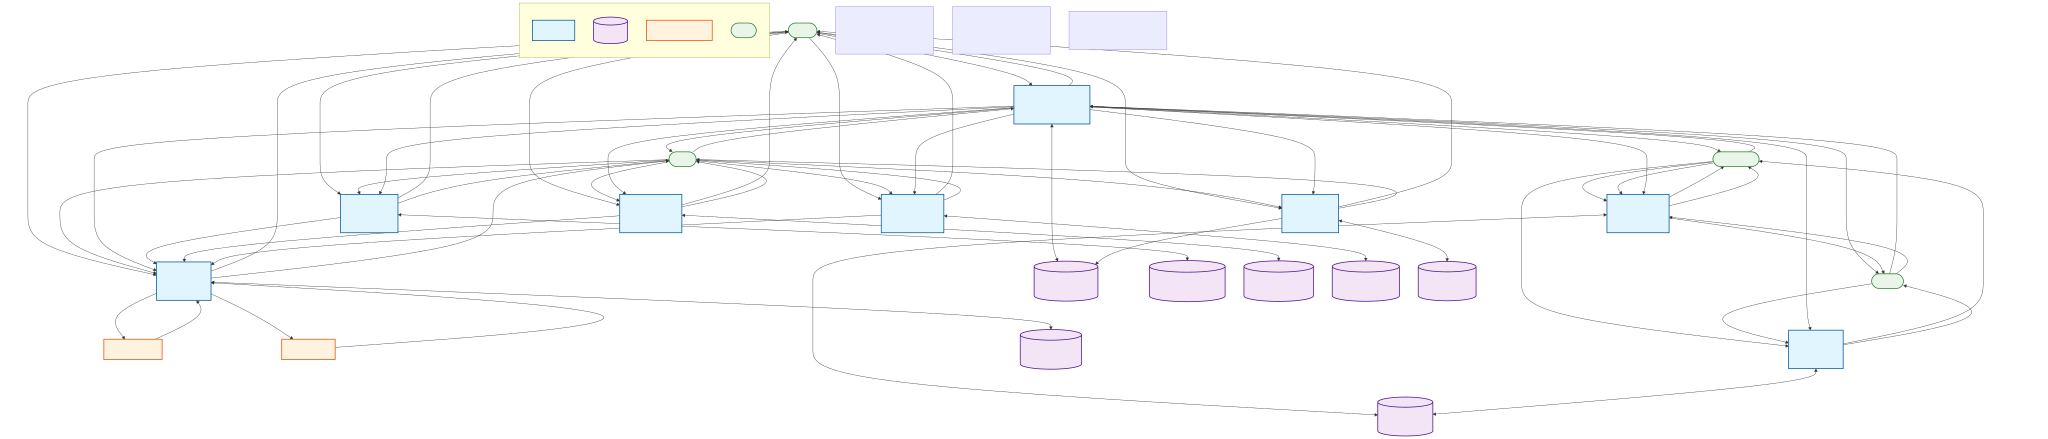
\includegraphics[width=0.9\textwidth]{diagrams/data_flow_diagram.png}
\caption{System Data Flow Diagram}
\label{fig:data-flow-diagram}
\end{figure}

\section{Requirement Specifications}

\subsection{Common functions}

\subsubsection{UC-01 – Register Donor Account}

\renewcommand{\arraystretch}{1.5}
\begin{longtable}{|p{4.5cm}|p{10.5cm}|}
\hline
\textbf{UC ID and Name:} & UC-01 – Register Donor Account \\
\hline
\textbf{Created By:} & DatNT \\
\hline
\textbf{Date Created:} & 28/6 \\
\hline
\textbf{Primary Actor:} & Guest \\
\hline
\textbf{Secondary Actors:} & System \\
\hline
\textbf{Description:} & A new user registers using email, password, and date of birth. The system creates a Level 1 account with the "Donor" role. To upgrade to Level 2 (eligible for blood donation registration), the user must visit a certified medical facility for in-person identity and eligibility verification. \\
\hline
\textbf{Trigger:} & The user clicks the 'Register' button. \\
\hline
\textbf{Preconditions:} &
\begin{itemize}
  \item The user is not logged in
  \item The email is not already in use
\end{itemize} \\
\hline
\textbf{Postconditions:} &
\begin{itemize}
  \item A Level 1 donor account is created
  \item The user can log in
  \item The account remains ineligible for donation event registration until verified (Level 2)
\end{itemize} \\
\hline
\textbf{Normal Flow:} &
\begin{enumerate}
  \item User opens the registration page
  \item Fills in the form
  \item Submits the form
  \item System validates input and creates the account
\end{enumerate} \\
\hline
\textbf{Alternative Flows:} & None defined \\
\hline
\textbf{Exceptions:} &
\begin{itemize}
  \item EX-1: If the email is already in use, the system shows an error message: \textit{"Email is already in use. Please use another email."}
  \item EX-2: If the user is under the required age, the system shows an ineligibility message: \textit{"You are not eligible to register as a blood donor."}
  \item EX-3: If a database or server error occurs, the system shows a retry message: \textit{"A system error occurred. Please try again later."}
\end{itemize} \\
\hline
\textbf{Business Rules:} &
\begin{itemize}
  \item BR-21: Only Level 2 (verified) users can register for donation events
  \item BR-22: User profile must be accurate and match official documents (relevant for Level 2 verification)
\end{itemize} \\
\hline
\textbf{Assumptions:} &
\begin{itemize}
  \item The user provides a valid email and basic profile information
  \item Level 2 access requires identity and health status confirmation at a medical center
\end{itemize} \\
\hline
\textbf{Priority:} & High \\
\hline
\textbf{Frequency of Use:} & Daily \\
\hline
\end{longtable}





\subsubsection{UC-02 – Log In}


\renewcommand{\arraystretch}{1.5}
\begin{longtable}{|p{4.5cm}|p{10.5cm}|}
\hline
\textbf{UC ID and Name:} & UC-02 – Log In \\
\hline
\textbf{Created By:} & KhoaDD \\
\hline
\textbf{Date Created:} & 28/6 \\
\hline
\textbf{Primary Actor:} & Guest, Donor \\
\hline
\textbf{Secondary Actors:} & System \\
\hline
\textbf{Description:} & The user logs into the system using their email and password. Upon successful login, the system redirects the user to their personal dashboard. Account access may be limited based on verification level (Level 1 or Level 2). \\
\hline
\textbf{Trigger:} & The user submits the login form. \\
\hline
\textbf{Preconditions:} &
\begin{itemize}
  \item A registered account exists
  \item The user is not currently logged in
\end{itemize} \\
\hline
\textbf{Postconditions:} &
\begin{itemize}
  \item The user is authenticated
  \item The user is redirected to their personal dashboard
\end{itemize} \\
\hline
\textbf{Normal Flow:} &
\begin{enumerate}
  \item User opens the login form
  \item Enters email and password
  \item Submits the form
  \item The system validates the credentials and logs the user in
  \item User is redirected to the dashboard with access based on account verification level
\end{enumerate} \\
\hline
\textbf{Alternative Flows:} & None defined \\
\hline
\textbf{Exceptions:} &
\begin{itemize}
  \item EX-1: If the email or password is incorrect, show an error message: \textit{"Invalid email or password."}
  \item EX-2: If the system is unavailable (e.g., server error), show an error message: \textit{"Unable to connect. Please try again later."}
\end{itemize} \\
\hline
\textbf{Business Rules:} &
\begin{itemize}
  \item BR-24: Email must follow institutional format (e.g., *@gmail.com)
\end{itemize} \\
\hline
\textbf{Assumptions:} &
\begin{itemize}
  \item The account is active and verified
  \item The user provides correct credentials
\end{itemize} \\
\hline
\textbf{Priority:} & High \\
\hline
\textbf{Frequency of Use:} & Daily \\
\hline
\end{longtable}

\subsubsection{UC-03 – View Hospital Information}

\renewcommand{\arraystretch}{1.5}
\begin{longtable}{|p{4.5cm}|p{10.5cm}|}
\hline
\textbf{UC ID and Name:} & UC-03 – View Hospital Information \\
\hline
\textbf{Created By:} & AnPP \\
\hline
\textbf{Date Created:} & 28/6 \\
\hline
\textbf{Primary Actor:} & Guest \\
\hline
\textbf{Secondary Actors:} & None \\
\hline
\textbf{Description:} & The user views information about the hospital, including its services, location, and contact details. \\
\hline
\textbf{Trigger:} & The user accesses the homepage or selects the "About Us" section. \\
\hline
\textbf{Preconditions:} &
\begin{itemize}
  \item The system is online and accessible
\end{itemize} \\
\hline
\textbf{Postconditions:} &
\begin{itemize}
  \item Hospital information is displayed to the user
\end{itemize} \\
\hline
\textbf{Normal Flow:} &
\begin{enumerate}
  \item User opens the website
  \item Clicks on "About Us"
  \item The system displays hospital information
\end{enumerate} \\
\hline
\textbf{Alternative Flows:} & None defined \\
\hline
\textbf{Exceptions:} &
\begin{itemize}
  \item EX-1: If hospital data is unavailable, the system displays a default message or an error: \textit{"Hospital information is currently unavailable."}
\end{itemize} \\
\hline
\textbf{Business Rules:} &
\begin{itemize}
  \item BR-19: Only admins can make changes to system about hospital information
\end{itemize} \\
\hline
\textbf{Assumptions:} &
\begin{itemize}
  \item Hospital information is properly maintained and updated in the system
\end{itemize} \\
\hline
\textbf{Priority:} & Medium \\
\hline
\textbf{Frequency of Use:} & Occasional \\
\hline
\end{longtable}


\subsubsection{UC-04 – Read Blogs}

\renewcommand{\arraystretch}{1.5}
\begin{longtable}{|p{4.5cm}|p{10.5cm}|}
\hline
\textbf{UC ID and Name:} & UC-04 – Read Blogs \\
\hline
\textbf{Created By:} & AnPP \\
\hline
\textbf{Date Created:} & 29/6 \\
\hline
\textbf{Primary Actor:} & Guest \\
\hline
\textbf{Secondary Actors:} & System \\
\hline
\textbf{Description:} & The user reads educational blog posts related to blood donation. \\
\hline
\textbf{Trigger:} & The user clicks on the "Blog" section. \\
\hline
\textbf{Preconditions:} &
\begin{itemize}
  \item At least one blog post has been published
\end{itemize} \\
\hline
\textbf{Postconditions:} &
\begin{itemize}
  \item A list of blogs is displayed
  \item The user can read individual posts
\end{itemize} \\
\hline
\textbf{Normal Flow:} &
\begin{enumerate}
  \item User clicks "Blog"
  \item System displays list of available posts
  \item User selects and reads a blog
\end{enumerate} \\
\hline
\textbf{Alternative Flows:} &
\textbf{AF-1:} No blog posts available → Show message: \textit{"No blog content is currently available."} \\
\hline
\textbf{Exceptions:} &
\begin{itemize}
  \item EX-1: System error → Show message: \textit{"Unable to load blogs. Please try again later."}
\end{itemize} \\
\hline
\textbf{Business Rules:} &
\begin{itemize}
  \item BR-17: Only blog authors or admins can edit blog articles
\end{itemize} \\
\hline
\textbf{Assumptions:} &
\begin{itemize}
  \item Blog content is reviewed and approved before being published
\end{itemize} \\
\hline
\textbf{Priority:} & Medium \\
\hline
\textbf{Frequency of Use:} & Frequent \\
\hline
\end{longtable}


\subsubsection{UC-05 – Manage Personal Profile}

\renewcommand{\arraystretch}{1.5}
\begin{longtable}{|p{4.5cm}|p{10.5cm}|}
\hline
\textbf{UC ID and Name:} & UC-05 – Manage Personal Profile \\
\hline
\textbf{Created By:} & TuanTM \\
\hline
\textbf{Date Created:} & 28/6 \\
\hline
\textbf{Primary Actor:} & Donor \\
\hline
\textbf{Secondary Actors:} & System \\
\hline
\textbf{Description:} & The donor views and updates their personal profile, including contact information. \\
\hline
\textbf{Trigger:} & The user accesses the "My Profile" section. \\
\hline
\textbf{Preconditions:} &
\begin{itemize}
  \item The user is logged in to the system
\end{itemize} \\
\hline
\textbf{Postconditions:} &
\begin{itemize}
  \item Profile data is updated and saved successfully
\end{itemize} \\
\hline
\textbf{Normal Flow:} &
\begin{enumerate}
  \item User navigates to profile section
  \item Edits personal information
  \item Clicks "Save"
  \item System validates and saves changes
\end{enumerate} \\
\hline
\textbf{Alternative Flows:} &
\textbf{AF-1:} Invalid input (e.g., phone number format) → Show error: \textit{"Please correct the highlighted fields."} \\
\hline
\textbf{Exceptions:} &
\begin{itemize}
  \item EX-1: If update fails due to system error → Show error: \textit{"Failed to update profile. Please try again."}
\end{itemize} \\
\hline
\textbf{Business Rules:} &
\begin{itemize}
  \item BR-22: User profile information must be accurate and match official documents
\end{itemize} \\
\hline
\textbf{Assumptions:} &
\begin{itemize}
  \item Profile data is accurate and editable
\end{itemize} \\
\hline
\textbf{Priority:} & High \\
\hline
\textbf{Frequency of Use:} & Occasional \\
\hline
\end{longtable}


\subsubsection{UC-06 – View Dashboard}

\renewcommand{\arraystretch}{1.5}
\begin{longtable}{|p{4.5cm}|p{10.5cm}|}
\hline
\textbf{UC ID and Name:} & UC-06 – View Dashboard \\
\hline
\textbf{Created By:} & System Team \\
\hline
\textbf{Date Created:} & 28/6 \\
\hline
\textbf{Primary Actor:} & Patient \\
\hline
\textbf{Secondary Actors:} & System \\
\hline
\textbf{Description:} & Patients access their personal dashboard with overview of appointments and treatments. \\
\hline
\textbf{Trigger:} & User logs in and navigates to dashboard. \\
\hline
\textbf{Preconditions:} &
\begin{itemize}
  \item User is authenticated as patient
  \item User has active account
\end{itemize} \\
\hline
\textbf{Postconditions:} &
\begin{itemize}
  \item Dashboard displays current appointments
  \item Treatment status is visible
  \item Notifications are shown
\end{itemize} \\
\hline
\textbf{Normal Flow:} &
\begin{enumerate}
  \item User logs into system
  \item System displays patient dashboard
  \item User views appointments and treatments
  \item User can navigate to other features
\end{enumerate} \\
\hline
\textbf{Alternative Flows:} &
\textbf{AF-1:} No appointments scheduled → Show message: \textit{"No upcoming appointments."} \\
\hline
\textbf{Exceptions:} &
\begin{itemize}
  \item EX-1: Dashboard loading error → Show message: \textit{"Unable to load dashboard. Please try again."}
\end{itemize} \\
\hline
\textbf{Business Rules:} &
\begin{itemize}
  \item BR-24: Dashboard shows only patient's own data
\end{itemize} \\
\hline
\textbf{Assumptions:} &
\begin{itemize}
  \item Patient has valid login credentials
\end{itemize} \\
\hline
\textbf{Priority:} & High \\
\hline
\textbf{Frequency of Use:} & Very Frequent \\
\hline
\end{longtable}

\subsubsection{UC-07 – Book Appointment}

\renewcommand{\arraystretch}{1.5}
\begin{longtable}{|p{4.5cm}|p{10.5cm}|}
\hline
\textbf{UC ID and Name:} & UC-07 – Book Appointment \\
\hline
\textbf{Created By:} & System Team \\
\hline
\textbf{Date Created:} & 28/6 \\
\hline
\textbf{Primary Actor:} & Patient \\
\hline
\textbf{Secondary Actors:} & System, Doctor \\
\hline
\textbf{Description:} & Patients schedule appointments with available doctors based on doctor availability slots. \\
\hline
\textbf{Trigger:} & User clicks "Book Appointment" button. \\
\hline
\textbf{Preconditions:} &
\begin{itemize}
  \item User is authenticated as patient
  \item Doctors have available time slots
\end{itemize} \\
\hline
\textbf{Postconditions:} &
\begin{itemize}
  \item Appointment is scheduled
  \item Doctor's slot is marked as booked
  \item Notification is sent to patient and doctor
\end{itemize} \\
\hline
\textbf{Normal Flow:} &
\begin{enumerate}
  \item User selects doctor from available list
  \item User selects preferred date
  \item System shows available time slots
  \item User selects time slot
  \item User enters appointment notes (optional)
  \item User confirms booking
  \item System creates appointment record
\end{enumerate} \\
\hline
\textbf{Alternative Flows:} &
\textbf{AF-1:} No available slots → Show message: \textit{"No available slots for selected date."} \\
\hline
\textbf{Exceptions:} &
\begin{itemize}
  \item EX-1: Booking conflict → Show message: \textit{"Slot no longer available. Please select another."}
\end{itemize} \\
\hline
\textbf{Business Rules:} &
\begin{itemize}
  \item BR-25: No overlapping appointments for same patient
  \item BR-26: Appointments must be at least 24 hours in advance
\end{itemize} \\
\hline
\textbf{Assumptions:} &
\begin{itemize}
  \item Doctor availability is up-to-date
\end{itemize} \\
\hline
\textbf{Priority:} & High \\
\hline
\textbf{Frequency of Use:} & Frequent \\
\hline
\end{longtable}

\subsubsection{UC-08 – View Appointments}

\renewcommand{\arraystretch}{1.5}
\begin{longtable}{|p{4.5cm}|p{10.5cm}|}
\hline
\textbf{UC ID and Name:} & UC-08 – View Appointments \\
\hline
\textbf{Created By:} & System Team \\
\hline
\textbf{Date Created:} & 28/6 \\
\hline
\textbf{Primary Actor:} & Patient \\
\hline
\textbf{Secondary Actors:} & System \\
\hline
\textbf{Description:} & Patients view their scheduled, completed, and cancelled appointments with details. \\
\hline
\textbf{Trigger:} & User navigates to "My Appointments" section. \\
\hline
\textbf{Preconditions:} &
\begin{itemize}
  \item User is authenticated as patient
  \item User has appointment history
\end{itemize} \\
\hline
\textbf{Postconditions:} &
\begin{itemize}
  \item List of appointments is displayed
  \item Appointment details are accessible
\end{itemize} \\
\hline
\textbf{Normal Flow:} &
\begin{enumerate}
  \item User clicks "My Appointments"
  \item System retrieves appointment history
  \item System displays appointments by status
  \item User can view appointment details
\end{enumerate} \\
\hline
\textbf{Alternative Flows:} &
\textbf{AF-1:} No appointments found → Show message: \textit{"No appointments found."} \\
\hline
\textbf{Exceptions:} &
\begin{itemize}
  \item EX-1: Data retrieval error → Show message: \textit{"Unable to load appointments. Please try again."}
\end{itemize} \\
\hline
\textbf{Business Rules:} &
\begin{itemize}
  \item BR-27: Only show patient's own appointments
\end{itemize} \\
\hline
\textbf{Assumptions:} &
\begin{itemize}
  \item Appointment data is accurate and current
\end{itemize} \\
\hline
\textbf{Priority:} & High \\
\hline
\textbf{Frequency of Use:} & Frequent \\
\hline
\end{longtable}

\subsubsection{UC-09 – Cancel Appointment}

\renewcommand{\arraystretch}{1.5}
\begin{longtable}{|p{4.5cm}|p{10.5cm}|}
\hline
\textbf{UC ID and Name:} & UC-09 – Cancel Appointment \\
\hline
\textbf{Created By:} & System Team \\
\hline
\textbf{Date Created:} & 28/6 \\
\hline
\textbf{Primary Actor:} & Patient \\
\hline
\textbf{Secondary Actors:} & System, Doctor \\
\hline
\textbf{Description:} & Patients cancel scheduled appointments with cancellation reasons. \\
\hline
\textbf{Trigger:} & User clicks "Cancel" on scheduled appointment. \\
\hline
\textbf{Preconditions:} &
\begin{itemize}
  \item User is authenticated as patient
  \item Appointment exists and is scheduled
\end{itemize} \\
\hline
\textbf{Postconditions:} &
\begin{itemize}
  \item Appointment status is updated to cancelled
  \item Doctor's time slot becomes available
  \item Cancellation notification is sent
\end{itemize} \\
\hline
\textbf{Normal Flow:} &
\begin{enumerate}
  \item User selects appointment to cancel
  \item System shows cancellation confirmation
  \item User provides cancellation reason
  \item User confirms cancellation
  \item System updates appointment status
  \item System sends notifications
\end{enumerate} \\
\hline
\textbf{Alternative Flows:} &
\textbf{AF-1:} Appointment cannot be cancelled → Show message: \textit{"This appointment cannot be cancelled."} \\
\hline
\textbf{Exceptions:} &
\begin{itemize}
  \item EX-1: Cancellation too late → Show message: \textit{"Cancellation must be at least 2 hours before appointment."}
\end{itemize} \\
\hline
\textbf{Business Rules:} &
\begin{itemize}
  \item BR-28: Cancellation allowed up to 2 hours before appointment
\end{itemize} \\
\hline
\textbf{Assumptions:} &
\begin{itemize}
  \item Appointment is not already started
\end{itemize} \\
\hline
\textbf{Priority:} & Medium \\
\hline
\textbf{Frequency of Use:} & Occasional \\
\hline
\end{longtable}

\subsubsection{UC-10 – View Patient Records}

\renewcommand{\arraystretch}{1.5}
\begin{longtable}{|p{4.5cm}|p{10.5cm}|}
\hline
\textbf{UC ID and Name:} & UC-10 – View Patient Records \\
\hline
\textbf{Created By:} & System Team \\
\hline
\textbf{Date Created:} & 28/6 \\
\hline
\textbf{Primary Actor:} & Patient \\
\hline
\textbf{Secondary Actors:} & System \\
\hline
\textbf{Description:} & Patients access their own medical records, treatment history, and current medications. \\
\hline
\textbf{Trigger:} & User navigates to "Medical Records" section. \\
\hline
\textbf{Preconditions:} &
\begin{itemize}
  \item User is authenticated as patient
  \item Medical records exist for patient
\end{itemize} \\
\hline
\textbf{Postconditions:} &
\begin{itemize}
  \item Medical records are displayed
  \item Treatment history is accessible
\end{itemize} \\
\hline
\textbf{Normal Flow:} &
\begin{enumerate}
  \item User clicks "Medical Records"
  \item System retrieves patient's medical data
  \item System displays comprehensive records
  \item User can view different sections
\end{enumerate} \\
\hline
\textbf{Alternative Flows:} &
\textbf{AF-1:} No medical records → Show message: \textit{"No medical records found."} \\
\hline
\textbf{Exceptions:} &
\begin{itemize}
  \item EX-1: Access denied → Show message: \textit{"Unable to access medical records."}
\end{itemize} \\
\hline
\textbf{Business Rules:} &
\begin{itemize}
  \item BR-29: Patients can only view their own records
\end{itemize} \\
\hline
\textbf{Assumptions:} &
\begin{itemize}
  \item Medical records are up-to-date
\end{itemize} \\
\hline
\textbf{Priority:} & High \\
\hline
\textbf{Frequency of Use:} & Frequent \\
\hline
\end{longtable}

\subsubsection{UC-11 – Update Patient Records}

\renewcommand{\arraystretch}{1.5}
\begin{longtable}{|p{4.5cm}|p{10.5cm}|}
\hline
\textbf{UC ID and Name:} & UC-11 – Update Patient Records \\
\hline
\textbf{Created By:} & System Team \\
\hline
\textbf{Date Created:} & 28/6 \\
\hline
\textbf{Primary Actor:} & Patient \\
\hline
\textbf{Secondary Actors:} & System \\
\hline
\textbf{Description:} & Patients update their personal medical information and emergency contacts. \\
\hline
\textbf{Trigger:} & User clicks "Edit" on medical records page. \\
\hline
\textbf{Preconditions:} &
\begin{itemize}
  \item User is authenticated as patient
  \item Medical records exist for patient
\end{itemize} \\
\hline
\textbf{Postconditions:} &
\begin{itemize}
  \item Medical records are updated
  \item Changes are saved to database
\end{itemize} \\
\hline
\textbf{Normal Flow:} &
\begin{enumerate}
  \item User clicks "Edit Medical Records"
  \item System displays editable form
  \item User updates information
  \item User clicks "Save Changes"
  \item System validates and saves data
\end{enumerate} \\
\hline
\textbf{Alternative Flows:} &
\textbf{AF-1:} Invalid data → Show message: \textit{"Please correct the highlighted fields."} \\
\hline
\textbf{Exceptions:} &
\begin{itemize}
  \item EX-1: Save failed → Show message: \textit{"Unable to save changes. Please try again."}
\end{itemize} \\
\hline
\textbf{Business Rules:} &
\begin{itemize}
  \item BR-30: Only patient can update their own records
\end{itemize} \\
\hline
\textbf{Assumptions:} &
\begin{itemize}
  \item Patient provides accurate information
\end{itemize} \\
\hline
\textbf{Priority:} & Medium \\
\hline
\textbf{Frequency of Use:} & Occasional \\
\hline
\end{longtable}

\subsubsection{UC-12 – View ARV Treatments}

\renewcommand{\arraystretch}{1.5}
\begin{longtable}{|p{4.5cm}|p{10.5cm}|}
\hline
\textbf{UC ID and Name:} & UC-12 – View ARV Treatments \\
\hline
\textbf{Created By:} & System Team \\
\hline
\textbf{Date Created:} & 28/6 \\
\hline
\textbf{Primary Actor:} & Patient \\
\hline
\textbf{Secondary Actors:} & System \\
\hline
\textbf{Description:} & Patients view their HIV antiretroviral treatment regimens and adherence status. \\
\hline
\textbf{Trigger:} & User navigates to "ARV Treatments" section. \\
\hline
\textbf{Preconditions:} &
\begin{itemize}
  \item User is authenticated as patient
  \item ARV treatment records exist
\end{itemize} \\
\hline
\textbf{Postconditions:} &
\begin{itemize}
  \item ARV treatment history is displayed
  \item Current regimen is shown
  \item Adherence status is visible
\end{itemize} \\
\hline
\textbf{Normal Flow:} &
\begin{enumerate}
  \item User clicks "ARV Treatments"
  \item System retrieves treatment data
  \item System displays treatment regimens
  \item User can view adherence reports
\end{enumerate} \\
\hline
\textbf{Alternative Flows:} &
\textbf{AF-1:} No ARV treatments → Show message: \textit{"No ARV treatments found."} \\
\hline
\textbf{Exceptions:} &
\begin{itemize}
  \item EX-1: Data access error → Show message: \textit{"Unable to load ARV treatments."}
\end{itemize} \\
\hline
\textbf{Business Rules:} &
\begin{itemize}
  \item BR-31: Only show patient's own treatment data
\end{itemize} \\
\hline
\textbf{Assumptions:} &
\begin{itemize}
  \item Treatment data is current and accurate
\end{itemize} \\
\hline
\textbf{Priority:} & High \\
\hline
\textbf{Frequency of Use:} & Frequent \\
\hline
\end{longtable}

\subsubsection{UC-13 – View Doctor Dashboard}

\renewcommand{\arraystretch}{1.5}
\begin{longtable}{|p{4.5cm}|p{10.5cm}|}
\hline
\textbf{UC ID and Name:} & UC-13 – View Doctor Dashboard \\
\hline
\textbf{Created By:} & System Team \\
\hline
\textbf{Date Created:} & 28/6 \\
\hline
\textbf{Primary Actor:} & Doctor \\
\hline
\textbf{Secondary Actors:} & System \\
\hline
\textbf{Description:} & Doctors access their professional dashboard with patient appointments and notifications. \\
\hline
\textbf{Trigger:} & Doctor logs in and navigates to dashboard. \\
\hline
\textbf{Preconditions:} &
\begin{itemize}
  \item User is authenticated as doctor
  \item Doctor profile is active
\end{itemize} \\
\hline
\textbf{Postconditions:} &
\begin{itemize}
  \item Dashboard displays today's appointments
  \item Notifications are shown
  \item Quick actions are available
\end{itemize} \\
\hline
\textbf{Normal Flow:} &
\begin{enumerate}
  \item Doctor logs into system
  \item System displays doctor dashboard
  \item Doctor views appointments and notifications
  \item Doctor can navigate to other features
\end{enumerate} \\
\hline
\textbf{Alternative Flows:} &
\textbf{AF-1:} No appointments today → Show message: \textit{"No appointments scheduled for today."} \\
\hline
\textbf{Exceptions:} &
\begin{itemize}
  \item EX-1: Dashboard loading error → Show message: \textit{"Unable to load dashboard. Please try again."}
\end{itemize} \\
\hline
\textbf{Business Rules:} &
\begin{itemize}
  \item BR-32: Dashboard shows only doctor's own appointments
\end{itemize} \\
\hline
\textbf{Assumptions:} &
\begin{itemize}
  \item Doctor has valid login credentials
\end{itemize} \\
\hline
\textbf{Priority:} & High \\
\hline
\textbf{Frequency of Use:} & Very Frequent \\
\hline
\end{longtable}

\section{Design Specifications}

\subsection{Authentication System}

\subsubsection{User Login}

This screen allows users to authenticate into the system with role-based access to appropriate functionalities.

\textbf{Related use cases:} UC-002 User Login

\paragraph{UI Design}

\begin{longtable}{|p{3cm}|p{3cm}|p{8cm}|}
\hline
\textbf{Field Name} & \textbf{Field Type} & \textbf{Description} \\
\hline
Username* & Text Box & User enters registered username or email address for authentication \\
\hline
Password* & Password Box & User enters password (masked input for security) \\
\hline
Login & Button & Submits authentication request to server \\
\hline
Register & Hyperlink & Redirects to user registration page for new users \\
\hline
Forgot Password? & Hyperlink & Initiates password reset process \\
\hline
\end{longtable}

\paragraph{Database Access}

\begin{longtable}{|p{3cm}|p{2cm}|p{9cm}|}
\hline
\textbf{Table} & \textbf{CRUD} & \textbf{Description} \\
\hline
Users & R & Verify username/email and password hash for authentication \\
\hline
Roles & R & Retrieve user role information for authorization \\
\hline
LoginActivity & C & Log login attempt for security audit \\
\hline
\end{longtable}

\paragraph{SQL Commands}

\begin{lstlisting}[language=SQL]
-- 1. Authenticate user credentials
SELECT u.UserID, u.Username, u.Email, u.IsActive, r.RoleName
FROM Users u 
INNER JOIN Roles r ON u.RoleID = r.RoleID
WHERE (u.Username = ? OR u.Email = ?) AND u.IsActive = 1

-- 2. Log login activity
INSERT INTO LoginActivity 
(UserID, UsernameAttempted, AttemptTime, IsSuccess, IPAddress, UserAgent)
VALUES (?, ?, GETDATE(), ?, ?, ?)
\end{lstlisting}

\subsection{Appointment Management}

\subsubsection{Appointment Booking}

This screen enables patients to book appointments with available doctors by selecting from available time slots.

\textbf{Related use cases:} UC-004 Book Appointment

\paragraph{UI Design}

\begin{longtable}{|p{3cm}|p{3cm}|p{8cm}|}
\hline
\textbf{Field Name} & \textbf{Field Type} & \textbf{Description} \\
\hline
Doctor Selection* & Dropdown & List of available doctors with specialties \\
\hline
Appointment Date* & Date Picker & Calendar widget for selecting appointment date \\
\hline
Available Time Slots* & Radio Buttons & Dynamic list of available time slots for selected doctor/date \\
\hline
Appointment Notes & Text Area & Optional notes about appointment purpose or concerns \\
\hline
Book Appointment & Button & Submit appointment booking request \\
\hline
Cancel & Button & Return to previous screen without booking \\
\hline
\end{longtable}

\paragraph{Database Access}

\begin{longtable}{|p{3cm}|p{2cm}|p{9cm}|}
\hline
\textbf{Table} & \textbf{CRUD} & \textbf{Description} \\
\hline
Users & R & Retrieve available doctors with their specialties \\
\hline
DoctorAvailabilitySlots & R,U & Query available slots and mark as booked \\
\hline
Appointments & C & Create new appointment record \\
\hline
Notifications & C & Schedule appointment reminder notifications \\
\hline
\end{longtable}

\paragraph{SQL Commands}

\begin{lstlisting}[language=SQL]
-- 1. Get available doctors
SELECT u.UserID, u.FirstName, u.LastName, dp.Bio, s.SpecialtyName
FROM Users u
INNER JOIN DoctorProfiles dp ON u.UserID = dp.UserID
LEFT JOIN Specialties s ON dp.SpecialtyID = s.SpecialtyID
WHERE u.RoleID = (SELECT RoleID FROM Roles WHERE RoleName = 'Doctor')
AND u.IsActive = 1

-- 2. Get available time slots
SELECT AvailabilitySlotID, SlotDate, StartTime, EndTime
FROM DoctorAvailabilitySlots
WHERE DoctorUserID = ? AND SlotDate = ? AND IsBooked = 0
ORDER BY StartTime

-- 3. Create appointment
INSERT INTO Appointments 
(PatientUserID, DoctorUserID, AvailabilitySlotID, AppointmentDateTime, 
 Status, AppointmentNotes, CreatedAt, UpdatedAt)
VALUES (?, ?, ?, ?, 'Scheduled', ?, GETDATE(), GETDATE())

-- 4. Update availability slot
UPDATE DoctorAvailabilitySlots 
SET IsBooked = 1, UpdatedAt = GETDATE()
WHERE AvailabilitySlotID = ?
\end{lstlisting}

\subsection{Patient Care System}

\subsubsection{Patient Records Management}

This screen provides comprehensive medical record management for HIV patients including treatment history and current medications.

\textbf{Related use cases:} UC-007 Manage Patient Records

\paragraph{UI Design}

\begin{longtable}{|p{3cm}|p{3cm}|p{8cm}|}
\hline
\textbf{Field Name} & \textbf{Field Type} & \textbf{Description} \\
\hline
Medical History & Text Area & Comprehensive medical history including HIV diagnosis details \\
\hline
Current Allergies & Text Area & Known allergies and adverse reactions \\
\hline
Current Medications & Text Area & List of current medications including ARV regimens \\
\hline
Blood Type & Dropdown & ABO blood type classification \\
\hline
Emergency Contact & Text Box & Emergency contact person name \\
\hline
Emergency Phone & Text Box & Emergency contact phone number \\
\hline
Clinical Notes & Text Area & Doctor's clinical observations and notes \\
\hline
Save Record & Button & Save medical record updates \\
\hline
View ARV Treatments & Button & Access HIV treatment management screen \\
\hline
\end{longtable}

\paragraph{Database Access}

\begin{longtable}{|p{3cm}|p{2cm}|p{9cm}|}
\hline
\textbf{Table} & \textbf{CRUD} & \textbf{Description} \\
\hline
PatientRecords & R,U & Retrieve and update patient medical records \\
\hline
ARVTreatments & R & Access HIV treatment history \\
\hline
MedicationRoutines & R & View current medication schedules \\
\hline
Users & R & Verify doctor access permissions \\
\hline
\end{longtable}

\paragraph{SQL Commands}

\begin{lstlisting}[language=SQL]
-- 1. Retrieve patient record
SELECT RecordID, PatientUserID, MedicalHistory, Allergies, 
       CurrentMedications, BloodType, EmergencyContact, 
       EmergencyPhone, Notes, UpdatedAt
FROM PatientRecords
WHERE PatientUserID = ?

-- 2. Update patient record
UPDATE PatientRecords
SET MedicalHistory = ?, Allergies = ?, CurrentMedications = ?,
    BloodType = ?, EmergencyContact = ?, EmergencyPhone = ?,
    Notes = ?, UpdatedAt = GETDATE()
WHERE PatientUserID = ?

-- 3. Get ARV treatment history
SELECT ARVTreatmentID, Regimen, StartDate, EndDate, 
       Adherence, SideEffects, IsActive
FROM ARVTreatments
WHERE PatientUserID = ?
ORDER BY StartDate DESC
\end{lstlisting}

\section{Appendix}

\subsection{Assumptions \& Dependencies}

\begin{itemize}
    \item \textbf{AS-1:} Microsoft SQL Server database is available and properly configured for healthcare data storage
    \item \textbf{AS-2:} SMTP email service is configured for sending appointment and medication reminders
    \item \textbf{AS-3:} System users have basic computer literacy and internet access
    \item \textbf{AS-4:} Clinic staff will receive training on HIV patient management workflows
    \item \textbf{DE-1:} Integration with existing hospital information systems may be required
    \item \textbf{DE-2:} HIPAA compliance requirements must be met for patient data protection
    \item \textbf{DE-3:} System depends on reliable internet connectivity for real-time operations
\end{itemize}

\subsection{Limitations \& Exclusions}

\begin{itemize}
    \item System does not include billing or insurance processing capabilities
    \item Laboratory result integration is not included in current scope
    \item Telemedicine or video consultation features are excluded
    \item Mobile application development is not part of initial release
    \item Integration with pharmacy systems for prescription management is excluded
    \item Advanced analytics and reporting dashboards are limited in scope
\end{itemize}

\subsection{Business Rules}

\begin{longtable}{|p{2cm}|p{3cm}|p{9cm}|}
\hline
\textbf{ID} & \textbf{Category} & \textbf{Rule Definition} \\
\hline
BR-016 & Data Security & All patient data must be encrypted at rest and in transit using AES-256 encryption \\
\hline
BR-017 & Access Control & Role-based access ensures patients can only view their own records unless explicitly shared \\
\hline
BR-018 & Appointment Scheduling & No overlapping appointments allowed for any doctor or patient \\
\hline
BR-019 & Medication Adherence & ARV medication reminders are mandatory for all HIV patients unless opted out \\
\hline
BR-020 & Record Retention & Patient medical records must be retained for minimum 7 years per healthcare regulations \\
\hline
BR-021 & Emergency Access & Emergency override allows authorized medical staff to access any patient record \\
\hline
BR-022 & Notification Preferences & Patients must be able to opt-out of non-critical notifications \\
\hline
BR-023 & Data Backup & Daily automated backups of all patient data with 30-day retention \\
\hline
\end{longtable}

\subsection{Technical Specifications}

\begin{itemize}
    \item \textbf{Backend Technology:} Spring Boot 3.x with Java 17
    \item \textbf{Frontend Technology:} React 18 with modern JavaScript (ES6+)
    \item \textbf{Database:} Microsoft SQL Server with T-SQL stored procedures
    \item \textbf{Authentication:} JWT (JSON Web Tokens) with BCrypt password hashing
    \item \textbf{API Architecture:} RESTful APIs with JSON data exchange
    \item \textbf{Security:} HTTPS/TLS encryption, CORS configuration, input validation
    \item \textbf{Deployment:} Containerized deployment ready (Docker compatible)
\end{itemize}

\end{document}